\section{One bad fit, many candidate causes}

A single failed registration (a smooth mass instead of an ant, as in
Chapter~\ref{ch:introduction}) can originate at any of six points in the
pipeline of Chapter~\ref{ch:pipeline}, and diagnosing it requires asking a
different question at each one (Figure~\ref{fig:one-bad-fit}): what evidence
is actually available in the scan; which anatomical structure a given region
of the template is meant to represent; what pose the model currently
assumes; which target point a given vertex should correspond to; whether the
model has enough freedom that a wrong correspondence can still be hidden
behind a locally plausible surface; and whether the optimiser can actually
reach the solution that scores best, even when one exists. The rest of this
chapter answers each of these questions in turn, using the synthetic
correspondence instrument built in \S\ref{sec:synthetic-instrument} as the
common measuring stick.

\begin{figure}[!htb]
\centering
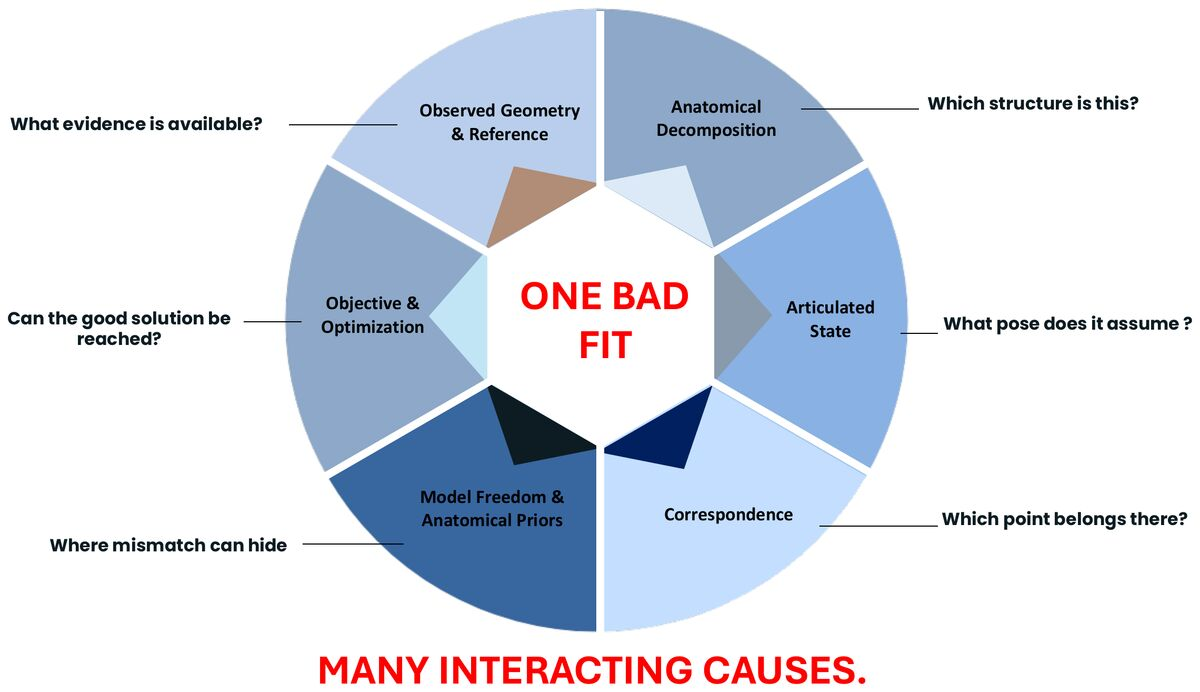
\includegraphics[width=0.55\linewidth]{figures/fig_one_bad_fit_wheel.jpg}
\caption{A bad fit is rarely attributable to a single cause. The six axes
investigated in this chapter interact, and an intervention aimed at one can
leave the anatomical failure it was meant to fix untouched (Chapter~\ref{ch:interventions}).}
\label{fig:one-bad-fit}
\end{figure}

Section~\ref{sec:three-failure-modes} closes the chapter with three
concrete failure modes that recur across the diagnostics below, each
surprising relative to the intuitive fix it might suggest.
